
Če želimo zasnovati asinhrona vezja moramo zasnovati visoko nivojski pogled, podobno kot pri sinhronih vezjih. Pri sinhronih vezjih je osnovna dogma to, da imamo zaporedje registrov in logike med njimi. Na vsak pozitivni rob urinega takta, se podatki prenesejo za en register naprej. To nam dovoli, da poenostavimo zasnovo sinhronih digitalnih vezji na zaporedje matematičnih operacij.

Podobno lahko storimo tudi pri asinhronih vezjih, imamo dodatne omejitve. Še vedno imamo zaporedje registrov, ter logiko med njimi, vendar se sedaj podatki ne pretakajo periodično, zato moramo zagotoviti da ne pride do zastojev.

\section{Protokoli} \label{a}

Najprej poglejmo kako podatke prenašamo skozi asinhrona vezja. Na sploh se protokoli deljio v dve skupini po dve skupini.

\subsection{Faznost} \label{b}

\begin{itemize}
	\item 2phase hitrejsi, ampak rabimo feedback da vemo kdaj smo done
	\item 4phase preprostejši več komunikacije
\end{itemize}

Pomislimo na mullerjev cevovod. Prenos podatkov po njem lahko gledamo na dva načina.
Lahko gledamo na nivoje signalov. Cikel torej gre reqdata, ackdata, reqnull, acknull. V tem pogledu potujeta skozi cevovod dva valova. Prvi je podatkovni val, ki prenaša podatke. Drugi je zaključni val, ki zakjuči komunikacijo, in spravi kanal v prvotno stanje.

Lahko gledamo robove signalov. Torej gledamo prenos dogodkov (pozitivni in negativni rob imata enak pomen). Torej gre samo za podatkovne valove, ki sledijo eden drugemu.


\subsection{Podatki} \label{b}

\begin{itemize}
	\item bundled data: Podoben sinhronim vezjem, potrebuje zakasnitve, da zagotovimo časovne predpostavke.
	\item Dual rail: Dve žici na bit, manj predpostavk
\end{itemize}

Do sedaj smo gledali cevovod le kot 1 biten podatkovni kanal. Vendar za procesiranje podatkov želimo več-bitne podatke. Cevovod lahko posplošimo na dva načina. 

Lahko signale, ki potujejo po cevovodu uporabimo, za odpiranje klasičnih registrov. To pomeni da lahko uporabimo klasične registre in klasično logiko. Vendar moramo paziti, da ohranimo pot skozi cevovod najdaljšo, torej potrebujemo zakasnilne elemente.

Lahko sklopimo več cevovodov skupaj. Med seboj moramo povezati povratne zanke in poskrbeti, za pravo kodiranje podatkov.

\subsubsection{Kodiranje} \label{b}
Kot vemo, moramo poskrbeti, da povratno zanko sinhroniziramo na najpočasnejši signal v zanki. To lahko zagotovimo z pravilnim kodiranjem podatkov. Koda je neodvisna od zakasnitev ko nobena kodna beseda ni vključena v drugi kodni besedi. Želimo tudi da je konkatanacija dveh kodnih besed nova kodna beseda.

Imamo dva jasna kandidata

\begin{itemize}
	\item One hot quad.
	\item Dual rail: One hot dual
\end{itemize}

One hot quad ima enako podatkovno gostoto kot dual rail, vendar ima pol manj preklopov, kar jo naredi bolj energisjko učinkovito. Vendar nismo še našli učinkovitih impelmentacij. Zato uporabimo Dual rail.

%
%A code (I ,C) is called delay-insensitive when :MATH @ dicodes:that is, when no code word is contained in another code word
%

Glede na gornje izbire dobimo 4 načine implementacije asinhronih vezji. Poglejmo si osnove vseh ter pogledjmo prednosti in slabosti.

\subsection{4-Phase bundled data} \label{b}
Ta stil je najbolj podoben klasični sinhroni logiki. Uporablja Mulerjev cevovod kot osnovno vodilo podatkovnega poteka. Na ta cevovod pripnemo navadne zapahe skozi katere pretekajo podatki. Med zapahe lahko vstavimo klasično logiko, a moramo paziti, da vsatvimo v Mullerjev cevovod zadostne zakasnitve, da zagotovimo dovolj časa, da se signali propagirajo skozi logiko. Ker je protokol 

\subsection{2-Phase bundled data} \label{b}
Ta stil je podoben 4-Phase bundled data, saj enako uporablja Mullerjev cevovod kot vodilo podatkov in klasično logiko. Ker uporablja 2 fazni protokol predstavljajo preklopi na cevovodu podatke o stanju cevovoda. Zato potrebujemo posebne zapahe, ki so odprti, ko sta stanja trenutne in naslednje stopnje cevovoda različni, sicer pa je zaprt. Tak protokol je hitrejši in bolj energetsko učikovit, prednost je tudi, da ne potrebujemo asimetričnih zakasnitev. Slabost so tudi posebni zapahi, ki niso del večine knjižnjic.

\subsection{4-Phase dual rail} \label{b}
Ta stil uporablja dual rail komunikacijo, kar prinese veliko overhead saj moramo uporabiti dvakrat več linij za podatkovne povezave in moramo vgraditi spominske celice v samo kombinatorično logiko. Druga stran je izjemna zanesljivost protokola, ki je dosežena popolnoma brez zakasnitev. Edina časovna predpostavka so nekatere isohronične veje, ki so zelo lahko izpolnjene

\subsection{2-Phase dual rail} \label{b}
Ta magisterska naloga se nanaša na implementacijo tega stila komunikacije. Je podoben 4-Phase dual rail, ampak namesto uporablja 2 fazni protokol, torej pridobimo na hitrosti in energijski učinkovitosti. Slabost je, da je povšina takšne izvedbe daleč največja. V nadaljnih poglavjih, se fokusiramo na prednosti in slabosti tega stila, ter njegovi detajli.




\section{Cevovodi} \label{a}

Cevovodi so osnovni arhitekturni element podatkovnega prenosa. Sestavljeni so iz zaporedja spominskih elementov, ki posredujejo podatke iz prejšnjega v naslednjega.

Glavno pravilo cevovodov je sledeče:
Register lahko shrani nov podatek od svojega prednjika, če je njegov naslednjik shranil podatek, ki ga trenutno vsebuje.

Osnovna implementacija enobitnega cevovoda v asinhronih vezjih je seveda Mullerjev cevovod. Če želimo cevovod posplošiti na več bitov lahko signalizacijo preprosto uporabimo za odpiranje navadnih registrov v bundled data stilu. 

Poglejmo si bolj detajlno posplošitev za dual rail sisteme.

Po Mullerjevem ceovodu, potujejo dogodki, ki pa nimajo vrednosti. Poglejmo si, kako poslati eno bitno vrednost.

Za to uporabimo dva vzporedna Mullerjeva cevovoda. Po enem bo tekel podatek za vrednost 0, po drugem podatek za vrednost 1. Povratni zanki obeh sihnalov moramo združiti, saj dobimo vedno signal le po eni izmed vej.

Implementacija 4fazne signalizacije, je veliko bolj preprosta kot 2fazne. Če uporabimo nadaljno transformacijo, lahko vezje poenstavimo. Izhodno vezje, je večbitna verzija Mousetrap vezja.Cite Mousetrap.

\begin{figure}
	\centering
	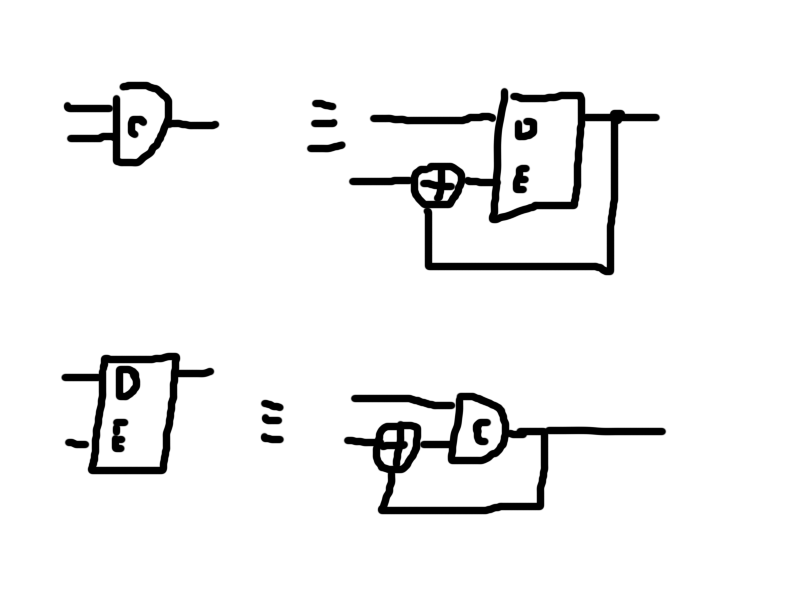
\includegraphics[width=0.7\linewidth]{slike/CtoD}
	\caption{}
	\label{fig:celement}
\end{figure}

Poglejmo si detejlno delovanje vezja. Sprememba pride po enem izmed cevovodov. Nato se sprememba propagira naprej, če je prostor in povratna informacija je poslana nazaj. V tej celotni verigi, Časovni zamiki niso važni za delovanje vezja. Vezje deluje pravilno po sami zasnovi (Seveda moramo biti pozorni na same časovne zahteve osnovnih elementov).

Tu spet vidimo veliko slabost dual rail, saj je potrebno več kot 2x več logike, za navaden cevovod.

Če želimo poslati večbiten podatek, uporabimo več enobitnih cevovodov. Povratne zanke skupaj vežemo s C elemnti, saj moramo tokrat sinhronizirati povratne zanke vseh enobitnih cevovodov.


%Linija iz knjige:
%A register may input and store a new data token from its predecessor if
%its successor has input and stored the data token that the register was pre-
%viously holding.
%
%Če pogledamo dano vezje lahko vidimo, da deluje kot 1-biten FIFO. Podatki se nalagajo noter in črpajo ven. Temu konstruktu se reče Mulerjev cevovod, in je osnova vseh asinhronih vezji.
%
%Lahko naredimo tudi obroče, Ali več sklenjenih obročov...
%
%Osnovna celica cevovoda je..., če pogledamo logične funkcije: ..., To lahko izvedemo tudi na druge načine.
%

\section{Logika} \label{a}

Logika je osnovni element podatkovnega procesiranja. Kot vhod ima dva ali več podatkov, kot izhod pa en podatek.
Kot vemo lahko vsa logična vezja implementiramo z NAND vrati, zato si poglejmo izdelavo NAND logičnih vrat.

V bundled data stilu, so NAND vrata implemntirana v klasičnem načinu npr CMOS. Poglejmo si implementacijo v dual rail stilu.

Osnovna ideja je podobna, kot implementacija klasičnih kombinatornih vezij z ALI/IN matriko. Najprej imamo detektor za vsako možno vhodno kombinacijo(IN), nato izhode teh detektorjev kombiniramo(ALI) skladno z našo pravilnostno tabelo.

Pri 4 phase stilu to implementiramo z uporabo C elementov za detektorje vhodne kombinacije in ali vrat za kombinacijo teh izhodov. Tu se je pomembno zavedati, da niso vse možne vhodne kombinacije veljavne in zato zaznavamo le kombinacije, ki so veljavne.

Pri 2-faznem stilu uporabimo podobno implementacijo, vendar moramo vhode C elementov sami ponastaviti, da ne ostanejo nekateri detektorji le delno aktivirani. To storimo z XOR vrati, ki jih postavimo za vhode. Ker vemo točno katera kombinacija vhodov je bila detektirana, lahko ponastavimo le tiste vhode, ki so bili aktivirani.

Za 4 fazna vezja obstaja tudi način optimizacije logičnih vezji citeNCL. 
V NCL logiki gledamo na C elemente in ALI vrata kot poseben primer N od M prestopnih vrat. S tem posplošenim naborom vrat lahko načrtamo kombinacijska vezja z veliko manjšim številom tranzistorjev oziroma v našem primeru, manjšim številom celic.



%I love U <3





\section{Podatkovni potek} \label{a}

Premikanje podatkov povezju je podatkovni potek. Za obravnavo podatkovnega poteka, nas zanimajo le registri, ter povezave med njimi, saj so logični elementi prozorni (podatke obdelajo, a ne vplivajo na njihovo pot skozi vezje).

V sekvenčnih vezjih se podatki premikajo iz enega zapaha v naslednjega.
 Footnote: Registri so narejeni iz para zapahov. Lahko uporabimo tudi samo zapahe in jih prožimo z alternirajočo fazo ure. Iz tega je razvidno, da za sinhrona vezja potrebijemo v ciklu vedno sodo število zapahov. 
Za pravilno delovanje mora vezje zagotavljati naslednjim zahtevam: 

\begin{itemize}
	\item Podatki ne izginjajo
	\item Podatki se ne pojavljajo iz nikoder
	\item Zaporedje podatkov je konsistentno.
\end{itemize}

Podatkovni pretok je pri asinhronih vezjih podoben kot pri sinhronih vezjih vendar obstajajo pomembne razlike. 
V sinhronih vezjih so v registrih vedno veljavni podatki in lahko se zanašamo na hitrost pretoka podatkov po vezju. Vsi podatki se ob urinem ciklu premaknejo za en register naprej.
V asinhronih vezjih potujejo podatki kot kot valovi. V eno smer potujejo valovi podatkov, v nasprotno smer pa potujejo valovi potrdil, ki signalizirajo sprembo podatkov. 

Število teh valov v vezju je pomembno, saj niso vse konfiguracije ustrezne. Če so na primer vsi zapahi zasedeni z podatki, se ne more noben podatek premakniti, kar ustavi celotno vezje. Če ni nobenega podatka, vezje jasno ne more delovati. Poglejmo si pravila ki jim vezja morajo slediti in pravila po katerih se podatki obnašajo v vezjih.


%Podatki se pretakajo po asinhronih vezjih kot valovi. v eno smer gre data, v drugo gre ACK. Vedno moramo kontrolirati število podatkovnih valov v vezju ect.
%To lahko gledamo kot graf po katerem se pretekajo tokeni. 
%
%Osnova igre ect:
%
%Drugače za 2 phase kot za 4 phase:

\subsection{Gradniki} \label{b}
Logični potek vezji gradimo iz majhne skupine gradnikov, ki zagotavljajo možnost zasnove velike večine vezji.


\subsubsection{Registri, izvori in ponori} \label{c}
Registri so glavni del vezja, ki diktirajo potek podatkov. 
Linearnem zaporedju registrov rečemo cevovod. Cevovodi služijo obdelavi podatkov v večih stopnjah tako, da med njih damo logične bloke, ali pomnilniku, da naredimo pretok podatkov skozi vezje bolj fleksibilno.
Zaporedju registrov, kjer je zadnji register v zaporedju povezan z prvim pravimo obroč. Take strukture so uporabne za iterativne izračune.

Izvori so viri podatkov. Ko dobijo potrdiev generirajo podatek. Ponori so nasprotje, vhodne podatke zavžejo in oddajo potrditev. Izvori in ponori pogosto prestavljajo mejo med vezjem in okoljem a ne vedno. Izvori predstavljajo tudi npr. konstante.

\subsubsection{Podvojitve in sinhronizacija} \label{c}
Podvojitve so deli vezja, kjer je podatek dupliciran in posredovan dvema registroma. Potrditve slednjih registrov sta združeni, torej potrebujemo potrditev obeh nadaljnih pretokov.
Sinhraonizacija je nasprotna operacija, kjer se dva podatka združita v enega. Tu čakamo, da so prisotni vsi vhodni podatki, preden nadaljujemo. Tu so ponavadi logični bloki.


\subsubsection{Razcepi in sponi} \label{c}
Razcepi so del vezji, kjer en podatkovni tok narekuje pot drugemu podatkovnemu toku. Je podoben multiplekserju, vendar multiplekser odda na vseh izhodih podatke (na ne izbranih izhodih je podatek 0) medtem, ko razcep posreduje podatek na le en izhod.

Spon je obratna operacija, kjer se dva pretoka podatkov združita. Tu ne čakamo vseh virov, vsak podatek preprosto posredujemo naprej.


\subsection{2phase} \label{b}
V dvofaznih protokolih, se v vezju pretakajo le podatkov. Vsak cikel mora imeti vsakj dva zapaha. Enega za podatkovni val in drugega, v katerega se podatkovni val premakne.

\subsection{4phase} \label{b}
Štirifazni protokoli so sicer identični dvofaznim, z razliko, da se po vezju pretakajo pari podatkov in ponastavitev. Iz tega razloga potrebuje vsak cikel vsaj 3 registre. Enega za podatek, enega za ponastavitev in enega, ki je prazen, da se vanj premakne podatek oz. ponastavitev.

\subsection{Inicializacija} \label{b}
Inicializacija vezja je vredna bližjega pogleda.
Če v inicaliziranem vezju ni podatkovnih valov lahko vezje preprosto inicializiramo tako, da vse spominske elemente postavimo na 0.

Če pa imamo v inicaliziranem vezju podatkovne valove, moramo poskrbeti za pravilno inicializacijo zapahov in povratnih zank. TODO add specifics maybe or cut


